\section{Design and Implementation}\label{sec:design}

Traditionally, game servers have been implemented much like game
clients. They are based around a main loop, which updates every active
element in the game.  These elements include for example player characters,
non-player characters and projectiles. The simulated world has a list
of all the active elements in the game, and typically calls an
"update" method on each element. In this method, the active element
will perform all its actions for the time-slot. 
Since these are sequential operations all actions can be performed directly. The
character reads input from the network, performs updates on itself
according to the input, and updates other elements with the results of
its actions.

To make a parallel game server with minimal locking, the system needs
to be redesigned from the ground up with parallelism in mind.
\subsection{Parallel main loop}

\begin{figure}
\centering
\vspace{-3mm}
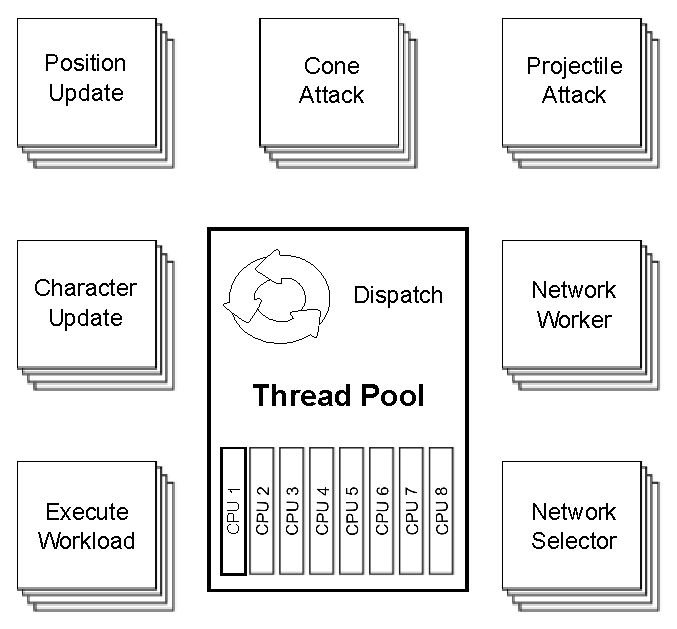
\psfig{file=FIG/server.eps,width=7.5cm}
\vspace{-2.5mm}
\caption{Design of the Game Server}
\vspace{-2.5mm}
\label{fig:server}
\vspace{-2.5mm}
\end{figure}

The system demonstrated here uses a threadpool executor as the core of
the main loop.  When an active element is created in the world, it
is scheduled for execution by the thread pool executor. When it
executes, the active element updates its state exactly as in the
single threaded case. When the task is finished for one time slot, it
can reschedule itself for the next slot, delayed by a specified time.
This allows active elements to have any lifetime from one-shot
executions to the duration of the program. It also allows different
elements to be updated at different rates, depending on the
requirements of the game developer.

The demo setup allows the user to interactively change the number of
threads in the threadpool. By setting the number of threads below the
number of cores it is, by means of the real-time monitoring, possible
to examine how well the cores are utilized.


\subsection{Use of locking}
The thread pool executor used as described above does not constrain
which tasks are executed in parallel. Therefore, all systems elements
must allow any of the other elements to execute concurrently. This
places one simple constraint on what an element can do; i.e., 
\emph{Elements can only update their own state, but read any state.}

This is sufficient because there is no need to establish consistent
ordering of events. This might sound counter intuitive, but it works since
the gameworld already is a simple simulation with a whole series of
approximations. All clients are connected to the server through
individual network links, with vastly different latencies.  The
clients are also run on different computers, with different update
frequencies. If player A performs an action slightly before player B,
this ordering is not necessarily kept by the server in the multi-threaded 
case. Running client update requests in parallel does not
aggravate this problem.

Another potential reason for locking is to keep state changes
atomic. This is also unnecessary due to the nature of the
problem. Consider the following example: Character A moves while
character B attacks. If only the X coordinate of character A is
updated at the point in time when the attack is executed, the attack
will see character A at position $(X_{t+\Delta T},Y_{t})$. This
position is within the accuracy of the simulation which in any case is
no better than the distance an object can move within the timeline $\Delta T$. The
only requirement for this to work is that assignment operations are
atomic.

The end result of our proposed design philosophy is that there is no
synchronization in the server under normal running conditions.

\subsection{Message passing}
Blocking queues~\cite{java:blockingqueue} are queue implementations
that are synchronized separately at each end. This means that elements
can be removed from the queue simultaneously with elements being
added. Each of these operations is also extremely quick, so the
probability of blocking is low.

These are used by the implementation to allow information to be passed
between active objects. Each active object that can be influenced by
others has a blocking queue of messages. During its update, it will
read and process the pending messages from its queue. Other active
elements put messages in the queue to be processed when they need to
change the state of other elements in the game.


\section{Example Game}
 This demonstration uses an implementation of a very simple game which
nonetheless contains all typical elements of a full Massively Multiplayer
Online game, with the exception of persistent state. The game itself
is simple. Each player controls a small circle ("the character") with
an indicator for which direction they are heading. The characters are
moved around by pressing keyboard buttons. They also have two attacks:
One projectile and one instant area of effect attack. Both attacks are
aimed straight ahead. If an attack hits another player character, the
attacker gets a positive point, and the character that was hit gets a
negative point. This simple game provides examples of all the elements
of the design described above:\begin{itemize}
\item The player character is a long lifetime active object. It
  processes messages from clients, updates states and potentially
  produces other active objects (attacks). In addition to position,
  which all objects have, the player also has information about how
  many times it has been hit and how many times it has hit others as
  part of its state. The player character also has a message queue to
  receive messages from other active objects. At the end of its
  update, it will enqueue itself for the next update unless
  the client has disconnected.
\item The frontal attack is a one shot task that finds player
  characters in its designated area and sends messages to those hit so
  they can update their counters, as well as back to the attacking
  player informing about how many were hit.
\item The projectile is a short lifetime object that moves in the
  world, checks if it has hit anything and reschedules itself for
  another update, unless it has hit something or ran to the end of its
  range. The projectile can only hit one target.
\end{itemize}

Our implementation has no spatial partitioning, we are interested in the worst
case, hence the numbers presented in this paper assume all players can see each
other at all times. This means that the number of messages and interactions by
necessity grows by the number of clients squared.

To simulate workload that grow linearly with number of players, especially
collision checks with the ground and other static objects, we have included a
synthetic load. The synthetic load is designed to emulate collision checks with
a grid representing the ground in the virtual world. To achieve this, we have
created an array of floating point values representing a part of the gameworld.
For each scheduled update, each character has to perform a square operation on
a given number of elements in the array. The operation is seeded with a
randomly generated value in order to avoid runtime optimizations in the virtual
machine. Which elements are processed depends on the player's position in the
gameworld. How many array elements are processed determines the severity of the
load. By adding the synthetic load, the cache is dirtied and the game server
processes becomes more realistic compared to a large-scale MMORPG. The demo
setup allows the user to experiment with different levels of synthetic load.
